\chapter{Interfaz gráfica}
\label{cha:gui}
 
Hasta ahora, las herramientas de verificación y minería mostradas en este proyecto utilizaban interfaces de usuario poco amigables para usuarios inexpertos: a través de línea de comandos para la herramienta STLEval; o mediante código fuente en Python para la librería ParetoLib.

En este apartado proponemos un espacio donde el usuario tenga que simplemente adjuntar los fichero de datos y operaciones (o elegir la operación a realizar desde las opciones disponibles) para finalmente poder visualizar y descargar la salida de señales en forma gráfica.
 
\section{Librerías utilizadas}

Para el desarrollo de la parte gráfica de este proyecto hemos hecho uso de las librerías:
\begin{itemize}
\item \href{https://www.qt.io/qt-for-python}{PyQt}
\item Matplotlib
\item Pandas
\item Seaborn
\end{itemize}
 
\subsection{PyQt}
Esta librería está basada en la biblioteca gráfica QT y nos servirá para realizar el diseño de la aplicación. En nuestro caso optamos por un diseño simple de 2 columnas: En la parte izquierda tendremos los botones y opciones para importar los ficheros de señales y la especificación de la operación, además de un espacio adicional para otras operaciones nuevas a implementar en un futuro. Al lado derecho tendremos la visualización de las señales tratadas y la especificación STL importada.

\begin{figure}[htb]
\centering
  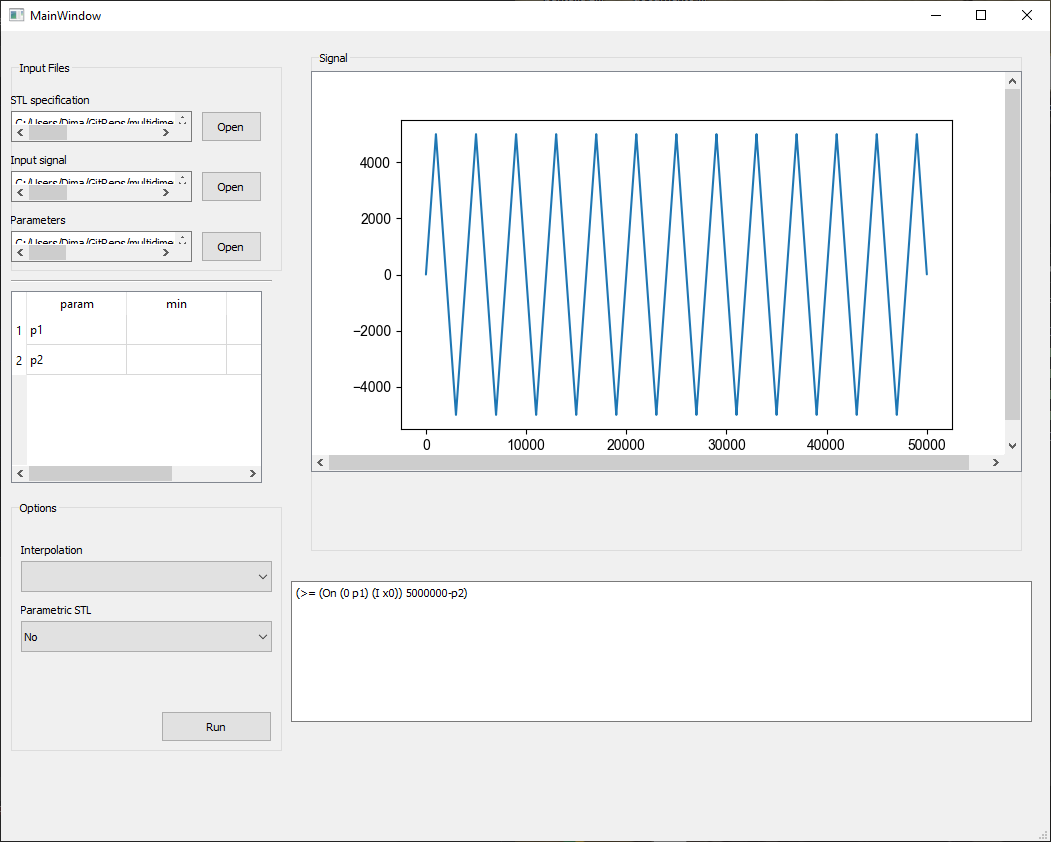
\includegraphics[width=1.0\linewidth]{images/gui} 
\caption{La ventana principal}
\label{fig:gui}
\end{figure}

%Instalación: 
%El desarrollo de la aplicación se hizo en un entorno linux haciendo uso del gestor de paquetes “pip”. 
 
%1 - Antes de todo, tenemos que confirmar la versión de Python que tenemos instalada con ´python3 --version´.
 
%2 - En el caso de que no lo tuviésemos, instalamos el gestor de paquetes “pip” con sudo ‘apt-get install python3-pip’ y actualizamos el mismo ´pip install -U pip´ 
 
%3 - Instalamos la librería PyQT con ´pip install pyqt5´. 
 
\subsection{MatplotLib}
Biblioteca usada para generar gráficos a partir de datos almacenados en un array. Hacemos uso de esta librería con el fin de mostrar las señales resultantes, aplicando las operaciones indicadas, en la sección de la aplicación propuesta para ello. 
 
%Instalación: 
 
%1 - En este caso es sumamente simple realizando: ´sudo apt-get install python3-matplotlib´.
 
\subsection{Pandas}
Librería de Python especializada en el manejo y análisis de estructuras de datos. En nuestro caso usada para la lectura de los ficheros csv, los cuales contienen los datos de entrada de las señales.
 
%Instalación: 
 
%1 - Instalamos la librería con el comando: ´pip install pandas´

\subsection{Seaborn} 
Basada en MatplotLib, es una librería que permite generar fácilmente elegantes gráficos. Nosotros la utilizamos para dibujar señales de los datos leídos de los archivos cvs.
 
%Instalación: 
 
%1 - Instalamos la librería con el comando: ´pip install seaborn´

\section{Estructura}
\begin{figure}[htb]
\centering
  \includegraphics[width=.95\linewidth]{images/uml_diagram} 
\caption{Estructura del proyecto}
\label{fig:est}
\end{figure}
Como vemos en la figura \ref{fig:est}, la GUI se comunica tanto con la librería de minería, que nos permite evaluar propiedades con o sin parámetros, como con la API STL. La librería de minería a su vez esta conectada por binarios precomplilados también con STL.

Las partes verdes de la estructura representan las partes nuevas de nuestra aportacion, como la propia GUI o los operadores nuevos de STL.
 
\section{Configuración Técnica}
El tratamiento de las señales se realiza mediante el consumo de la librería ParetoLib y el oráculo de STLe `ParetoLib.Oracle.OracleSTLe`. Las funciones de la API que utilizamos son: 
\begin{itemize}
\item OracleSTLeLib(stl\_prop\_file, csv\_signal\_file, stl\_param\_file): Constructor del objeto basado en la señal de entrada csv, sobre este objeto se van a realizar las operaciones del archivo de especificación que adjuntemos. 
\item \_load\_stl\_formula(stl\_file): Método que carga un archivo de especificación de la formula. 
\item eval\_stl\_formula(self, stl\_formula): Método que evalúa la fórmula y devuelve si es satisfacible.
\item \_get\_parameters\_stl(stl\_param\_file): Devuelve los parámetros del archivo dado como una lista.
%\item get\_var\_names(self):
\end{itemize} 

\section{Otros}
Cabe mencionar, que para sacar todo el potencial de PyQt5 hemos hecho uso de la herramienta Qt Designer. Gracias a ella hemos podido construir la interfaz en sí. Una vez hecha, la unimos al archivo GUI.py para aportar funcionalidades al propio diseño.
